\documentclass[11pt]{amsart}


\usepackage[ibidtracker=false,uniquename=false,giveninits=true,terseinits=true,backend=biber]{biblatex}
\usepackage{float}
\usepackage{graphicx}
\usepackage{todonotes}
\usepackage{subcaption}
\usepackage{amsmath}
\usepackage{amsthm}
\usepackage{amssymb}
\usepackage{algorithm}
\usepackage[noend]{algorithmic}
\usepackage[foot]{amsaddr}
\usepackage[misc]{ifsym}
\usepackage{enumitem}
\usepackage{geometry}
\usepackage[hidelinks]{hyperref}

\renewbibmacro{in:}{}
\addbibresource{rnni_geometry.bib}
\AtEveryBibitem{
	\clearlist{language}
}

\setlist{leftmargin = 0pt}
\geometry{margin=1in}


\newtheorem{proposition}{Proposition}
\newtheorem{theorem}{Theorem}
\newtheorem{lemma}{Lemma}
\newtheorem{corollary}{Corollary}
\newtheorem{problem}{Problem}
\newtheorem{conjecture}{Conjecture}

\newcommand{\lemmaautorefname}{Lemma}
\newcommand{\corollaryautorefname}{Corollary}
\renewcommand{\sectionautorefname}{Section}
\renewcommand{\subsectionautorefname}{Section}

\newcommand{\tocite}{ {\color{red}\fbox{CITATION}} }
\newcommand{\toref}{ {\color{blue}\fbox{Reference}} }
\newcommand{\rnni}{\mathrm{RNNI}}
\newcommand{\findpath}{\textsc{FindPath}}
\newcommand{\mrca}{\mathrm{mrca}}
\newcommand{\rank}{\mathrm{rank}}
\newcommand{\ntime}{\mathrm{time}}
\newcommand{\nni}{\mathrm{NNI}}
\newcommand{\spr}{\mathrm{SPR}}
\newcommand{\tbr}{\mathrm{TBR}}
\newcommand{\fp}{\mathrm{FP}}
\newcommand{\dtt}{\mathrm{DCT}}
\newcommand{\np}{\mathbf{NP}}
\newcommand{\decprob}[1]{\rnni(#1)\text{-}\mathrm{SP}}
\newcommand{\rad}{\mathit{rad}}
\renewcommand{\O}{\mathcal O}
\renewcommand{\epsilon}{\varepsilon}
\renewcommand{\thesubfigure}{\Alph{subfigure}}

\newcommand{\algorithmautorefname}{Algorithm}

% \newcommand{\summary}[1]{\textbf{#1}} % Print summaries to .pdf
\newcommand{\summary}[1]{} % Hide summaries in .pdf

\newcommand{\todefine}[1]{{\color{blue}{We need to define:#1}}} % Print summaries to .pdf

\DeclareMathOperator*{\argmin}{argmin}
\DeclareMathOperator*{\argmax}{argmax}

\graphicspath{{figures/}}

\sloppy


\title[Geometry of ranked tree spaces]{The Geometry of the space of Discrete Coalescent Trees}
\date{\today}
\author{Lena Collienne\textsuperscript{1}}
\email{lcollienne@cs.otago.ac.nz}
\address{\textsuperscript{1}Department of Computer Science, University of Otago, New Zealand}
\author{Kieran Elmes\textsuperscript{1}}
\email{kelmes@cs.otago.ac.nz}
\author{Mareike Fischer\textsuperscript{2}}
\email{email@mareikefischer.de}
\address{\textsuperscript{2}Institute of Mathematics and Computer Science, University of Greifswald, Germany}
\author{David Bryant\textsuperscript{3}}
\email{david.bryant@otago.ac.nz}
\address{\textsuperscript{3}Department of Mathematics and Statistics, University of Otago, New Zealand}
\author{Alex Gavryushkin\textsuperscript{1, \Letter}}
\email{\textsuperscript{\Letter}alex@biods.org}
\thanks{}


\begin{document}

\begin{abstract}
	Most methods for inferring phylogenetic trees base on tree search algorithm.
	Those algorithm require a tree space, which is often defined as a graph where trees are vertices and connected by an edge if one can be received from another by local changes to the tree, so-called tree-rearrangement operations.
	\todo[inline]{You need to talk about molecular clock here.}
	Often the goal is to reconstruct a tree where internal nodes, and hence speciation or divergence events, are equipped with times.
	This is especially the case in coalescence models, where the order of divergence events is of importance.
	Most classical tree-rearrangement operations like nearest neighbour interchange, subtree prune and regraft, or tree bisection and reconnection do not take the times of internal nodes into account.
	\todo[inline]{You don't need to go in such detail in the firs para of Intro.
	All these tree operations are technical things that can be mentioned towards the end of Intro.
	Here you can just say that treespaces exist for clock trees and we're considering one in this paper.}
	The ranked nearest neighbour interchange operations however, a generalisation of nearest neighbour interchange, considers ranked trees and thereby preserves the order of divergence events.

	\todo[inline]{Again, too details and shortest paths come out of the blue.
	Just say it was shown that the space has promising properties for statistical analyses in treespace.}
	It furthermore has recently been established that this space of ranked nearest neighbour interchange trees has shortest path that can be computed in polynomial time, unlike most other tree spaces.
	In this paper, we go gone step further and do not only consider ranked trees, but trees where nodes are assigned discrete coalescence times.
	We show that shortest paths in this space can be computed in polynomial time and establish some geometrical properties.
	Since the tree space considered in this paper can be seen as a generalisation of the space of ranked nearest neighbour interchange trees, most of our results apply to both tree spaces.
\end{abstract}

\maketitle


\section{Introduction}
\summary{Why we want a time-tree space}
\todo{This paragraph can be about molecular clock, then about a different parameterization necessary for inference software that deal with clock trees, and finally about tree proposals.
So possible two or three paragraphs.}
One of the main tasks in evolutionary biology is reconstructing evolutionary trees, also called phylogenetic trees, from various types of data, such as RNA or DNA sequences.
In order to gain knowledge about the evolutionary history in time, evolutionary trees where nodes are equipped with times are of interest in many applications, including research on cancer and virus evolution.
Most tree inference models for these problems, such as Maximum Likelihood \autocite{Kozlov2019-cf, Nguyen2015-sp, Tamura2011-ky} or Bayesian methods \autocite{Bouckaert2014-ir,Suchard2018-tw, Ronquist2003-eq}, rely on tree search algorithms.
These algorithms base on tree graphs where vertices represent trees that are connected by an edge if a local change, a so-called tree-rearrangement operation, transforms one tree to another.
Commonly used tree-rearrangement operations are nearest neighbour interchange, subtree prune and regraft, and tree bisection and reconnection.
None of these operations, however, take times of internal nodes of trees into account, and computing distances in the tree graphs basing on these operations is $\np$-hard \autocite{Dasgupta2000-xa, Bordewich2005-nx, Allen2001-ky, Hickey2008-wv}.

\summary{Why discrete coalescent trees}
\todo{This paragraph can be a description of coalescent as a popular class of evolutionary generating models, the parameterization should follow naturally after coalescent models are described.
So tree space is the last thing to appear, not first.}
It is hence desirable to have a tree space on trees where internal nodes, representing evolutionary events, are timed, and distances between trees can be computed in polynomial time.
This is in particular the case when trees are inferred using the coalescent model.
The coalescent model is popular for reconstructing genealogical trees to infer relationships of a sample of genes \autocite{Hudson1990-ki, Kuhner2009-jb}.
It is also widely used in population genetics, especially for estimating population dynamics \autocite{Kuhner1998-eh,Drummond2005-ak}.
Under the coalescent model, evolution is considered backwards in time.
The evolutionary history is hence derived from the time of the given samples back to its most recent common ancestor, resulting in trees where internal node are assigned unique times.
Commonly used reconstruction methods using MCMC \autocite{Bouckaert2014-ir,Suchard2018-tw} and Maximum Likelihood \autocite{Kozlov2019-cf, Nguyen2015-sp} implement the coalescent model to infer trees where nodes are assigned times, representing the times of the associated evolutionary events.

\summary{How recent results about $\rnni$ make this space interesting and that it is strongly connected to $\dtt_m$}
Therefore, tree spaces where internal nodes are assigned times are needed under the coalescent model.
\todo{BHV does not have time, and cannot be easily fixed to include molecular clock -- have a look at our paper with Alexei.}
Examples of such tree spaces include the BHV-space \autocite{Billera2001-rj}, t-space, and $\tau$-space \autocite{Gavryushkin2016-uu}, which parameterise trees in different ways.
The problem of these spaces is however, that there are no algorithms for computing shortest paths are known (t-space), or shortest paths lack biological meaningfulness.
More specifically, BHV space and the $\tau$-space suffer from having trees connected by unique geodesics that pass the star tree \autocite{Gavryushkin2016-uu}.
Summarising tree samples often results in star trees in these spaces, which do not contain any biological information.

\summary{Why we want to investigate geometrical properties of $\dtt_m$ and $\rnni$}
\todo{No, they don't -- it's the first time geometry is mentioned, so we need to link the discussion above to geometry.
Papers that employ geometric information in various algorithms and methods need to be cited here.
You sort of do it later on but I think a claim should follow an argument, unlike in maths :)}
This result highlights the importance of understanding geometrical properties of shortest paths in tree spaces.
Investigating those is essential for tree search algorithms, especially for developing these algorithms and evaluating inferred trees.
Methods estimating whether a chain converged in the bayesian tree inference approach, for example, rely on measuring distances between trees \autocite{Nylander2008-wa, Warren2017-df}.
Summarising a sample of trees, for example a posterior sample, also requires a tree space with efficiently computable distances, as well as shortest paths that preserve information shared between trees, in order to receive a biological meaningful summary tree.
Currently used methods for summarising trees do not rely on such tree spaces, as computing distances is $\np$-hard in most of them.
Instead, these methods use for example the Robinson-Foulds distance \autocite{Robinson1981-fb, Bansal2010-vr} to compute summary trees.
This distance can be computed efficiently, but lacks biological interpretability.
Alternatively, maximum clade credibility trees \autocite{Heled2013-sv} or consensus trees \autocite{Margush1981-ba} are used to summarise tree samples.
To compute biological meaningful summary trees where internal nodes are assigned times, it is therefore desirable to find a tree space where distances can be computed efficiently and shortest paths are biologically meaningful.

\summary{Structure of the paper.}
In this paper we consider the space $\dtt_m$ of discrete coalescent trees, where internal nodes are assigned distinct discrete times.
This space can be seen as a generalisation of the ranked nearest neighbour interchange ($\rnni$) space, which has been introduced by \textcite{Collienne2020-iu}.
We show in this paper that the space $\dtt_m$ has the desired properties mentioned above, including efficiently computable shortest paths that preserve biological information shared between trees.
After introducing notations used throughout this paper (\autoref{section:technical_introduction}), we discuss how the algorithm $\findpath$ \autocite{Collienne2020-iu} can be generalise from $\rnni$ to be applied to discrete coalescent trees, computing shortest paths in polynomial time (\autoref{section:fp_dtt}).
We then analyse some geometrical properties of both tree spaces $\dtt_m$ and $\rnni$ (\autoref{section:geometry}).
We do so by first discuss the cluster property in \autoref{section:cluster_property} and then considering a subset of trees (caterpillar trees) for which we are able to compute $\rnni$ distances even more efficiently than with $\findpath$ (\autoref{section:caterpillar_convex}).
Following that, we establish the diameter of $\dtt_m$ and $\rnni$ and briefly discuss the radius for each space.
We finish this paper with a section providing a connection between the $\rnni$ space and partition lattices, and propose directions for further research (\autoref{section:open_problems}).


\section{Technical Introduction}
\label{section:technical_introduction}

\summary{Introducing discrete coalescent trees and ranked trees}
A binary rooted phylogenetic tree is a binary tree on a fixed number $n$ of leaves, which are uniquely labelled by elements of the set $\{a_1, \ldots, a_n\}$.
The main objective of study in this paper are \emph{discrete coalescent trees}, binary rooted phylogenetic trees with positive integer-valued \emph{times} assigned to nodes.
More specifically, all leaves are assigned time $0$, and every internal node is assigned a unique time, such that it always has time greater than its children.
We denote the time of an internal node $v$ by $\ntime(v)$.
If not stated otherwise, we refer to discrete coalescent trees simply as \emph{trees}.
We furthermore call two trees (not necessarily binary) \emph{identical} if there is a graph isomorphism between them preserving leaf labels and times.
The number of discrete coalescent trees with root time less or equal to $m$ is $\frac{(n-1)!n!m^{n-1}}{2^{n-1}}$ \autocite{Gavryushkin2018-ol}.

As special case of discrete coalescent trees we consider \emph{ranked trees} with root time $n-1$.
In these trees internal nodes are uniquely labelled by times in $\{1, \ldots, n-1\}$.
This definition of ranked trees coincides with the one of \textcite{Collienne2020-iu}.
In the case of ranked trees we say \emph{rank} of a node $v$ to mean its time ($\rank(v) = \ntime(v)$) to be consistent with notations used in \autocite{Collienne2020-iu}.

Every internal node $v$ of a tree $T$ can be referred to by the set $C$ of leaves that are descending from this node.
We call such a set $C$ \emph{cluster} and say that the cluster $C$ is \emph{induced} by $v$.
A list of clusters $[C_1, \ldots, C_{n-1}]$ uniquely defines a ranked tree, where cluster $C_i$ is induced by the internal node with rank $i$ for $i \in \{1, \ldots, n-1\}$.
For discrete coalescent trees however, times of nodes also need to be provided to uniquely identify a tree.
For a subset $S \subseteq \{a_1, \ldots, a_n\}$ we call the internal node of a tree $T$ with lowest time among those ancestral to all elements of $S$ the \emph{most recent common ancestor} of $S$ and denote it by $(S)_T$.
We furthermore denote the parent of a leaf $a_i$ in $T$ by $(a_i)_T$, and the cluster induced by the node with time $i$ in $T$ by $(T)_i$.
An important type of trees that will be of importance throughout the whole paper are \emph{caterpillar trees}, which are trees where every internal nodes has at least one child that is a leaf.

\summary{Defining the tree space $\dtt_m$ and $\rnni = \dtt_{n-1}$}
We are now ready to introduce the central object of study of this paper, the graph (or space) of discrete coalescent trees.
This graph is called $\dtt_m$ for a fixed positive integer $m$.
The vertex set of $\dtt_m$ is the set of trees with root time less or equal to $m$.
Trees $T$ and $R$ are connected by an edge ($T$ and $R$ are \emph{neighbours}) in this graph if performing one of the following (reversible) operations on $T$ results in $R$:
\begin{enumerate}
	\item An \emph{$\nni$ move} connects trees $T$ and $R$ if there is an edge $e$ in $T$ and an edge $f$ in $R$, both of length one, such that shrinking $e$ and $f$ to nodes results in identical trees.
	\item A \emph{rank move} on $T$ exchanges the times of two internal nodes with time difference one.
	\item A \emph{length move} on $T$ changes the time of an internal node by one.
\end{enumerate}
A length move can only change the time of a node to become $t$ if there is no node with time $t$ already.
Note that our definition of $\dtt_m$ differs from the definition of \textcite{Gavryushkin2018-ol}, as length move are defined differently in their paper.

The definition of $\dtt_m$ leads to a natural definition of the \emph{distance} between two trees $T$ and $R$ in this graph as the length of a shortest paths between these trees, denoted by $d(T,R)$.
We also consider the ranked nearest neighbour interchange ($\rnni$) graph of \textcite{Collienne2020-iu}, which is the graph $\dtt_m$ for $m=n-1$, and hence a graph of ranked trees.
In this graph length moves are not possible, so we use the notion $\rnni$ \emph{move} to mean either a rank move or an $\nni$ move in order to distinguish these moves from length moves.


\section{Computing Shortest Paths in $\dtt_m$}
\label{section:fp_dtt}

\summary{Introduce how we can use $\findpath$ to compute $\dtt_m$ distances}
Shortest paths, and therefore distances, between trees in $\rnni$ can be computed with the algorithm $\findpath$, which was introduced by \textcite{Collienne2020-iu} and has running time quadratic in the number of leaves $n$.
As $\rnni$ is a special case of $\dtt_m$ for $m = n-1$, the question whether this algorithm can also be used to compute shortest paths in $\dtt_m$ arises.
In this section we present a generalisation of $\findpath$ that computes distances between trees in $\dtt_m$.
Before introducing the version of $\findpath$ for $\dtt_m$, we introduce a way to convert trees in $\dtt_m$ on $n$ leaves into ranked trees on $m+2$ leaves, such that the $\rnni$ distance between those ranked trees equals their distance in $\dtt_m$ (\autoref{thm:dtt_findpath}).

\summary{How to add leaves to a $\dtt_m$ tree to transform it into a ranked tree}
A tree $T$ in $\dtt_m$ on $n$ leaves can be converted into a ranked tree in $\rnni$ on $m+2$ in the following way (\autoref{alg:ranked_tree}).
First add a new root with time $m + 1$ that becomes parent of the root of $T$.
The second child of this new root is the root of a caterpillar tree on leaf set $\{a_{n+1}, a_{n+2}, \ldots, a_{m+2}\}$, such that $\ntime(a_{n+1}) = \ntime(a_{n+2}) < \ntime(a_{n+3}) < \ldots < \ntime(a_{m+2})$.
The resulting tree $T_r$ is hence a uniquely defined ranked tree with $m+2$ leaves.
An example of this extension of a tree $T$ to a ranked tree $T_r$ is depicted in \autoref{fig:dtt_to_ranked_tree}.

Throughout this paper we use the index $r$ to refer to this extended ranked version $T_r$ of a tree $T$.
Moreover, we denote the subtree of $T_r$ that is identical to $T$ by $T_r^d$ ($d$ for discrete coalescent tree) and the caterpillar subtree on leaf set $\{a_{n+1}, \ldots, a_{m+2}\}$ by $T_r^c$.

\begin{algorithm}[ht]
	\caption{RankedTree($T$, $m$)}
	\label{alg:ranked_tree}
	\begin{algorithmic}[1]
		\STATE $S:= \{1 \leq i \leq m | \text{ no internal node in } T \text{ has time } i\}$
		\STATE $[i_1, \ldots, i_{m-n+1}] = sort(S)$
		\STATE $T_r^d =$ copy of $T$
		\STATE $T_r^c =$ tree consisting of just one internal node $v_1$ with rank $i_1$ and children $a_{n+1}, a_{n+2}$
		\FOR {$k = 2, \dots, m-n+1$}
			\STATE Add internal node $v_k$ with with time $i_k$ and children $v_{k-1}$ and $a_{n+1+k}$ to $T_r^c$
		\STATE $T_r = $ tree with root with time $m+1$ and children of root are roots of $T_r^d$ and $T_r^c$.
		\ENDFOR
		\RETURN $T_r$
	\end{algorithmic}
\end{algorithm}

\begin{figure}[ht]
	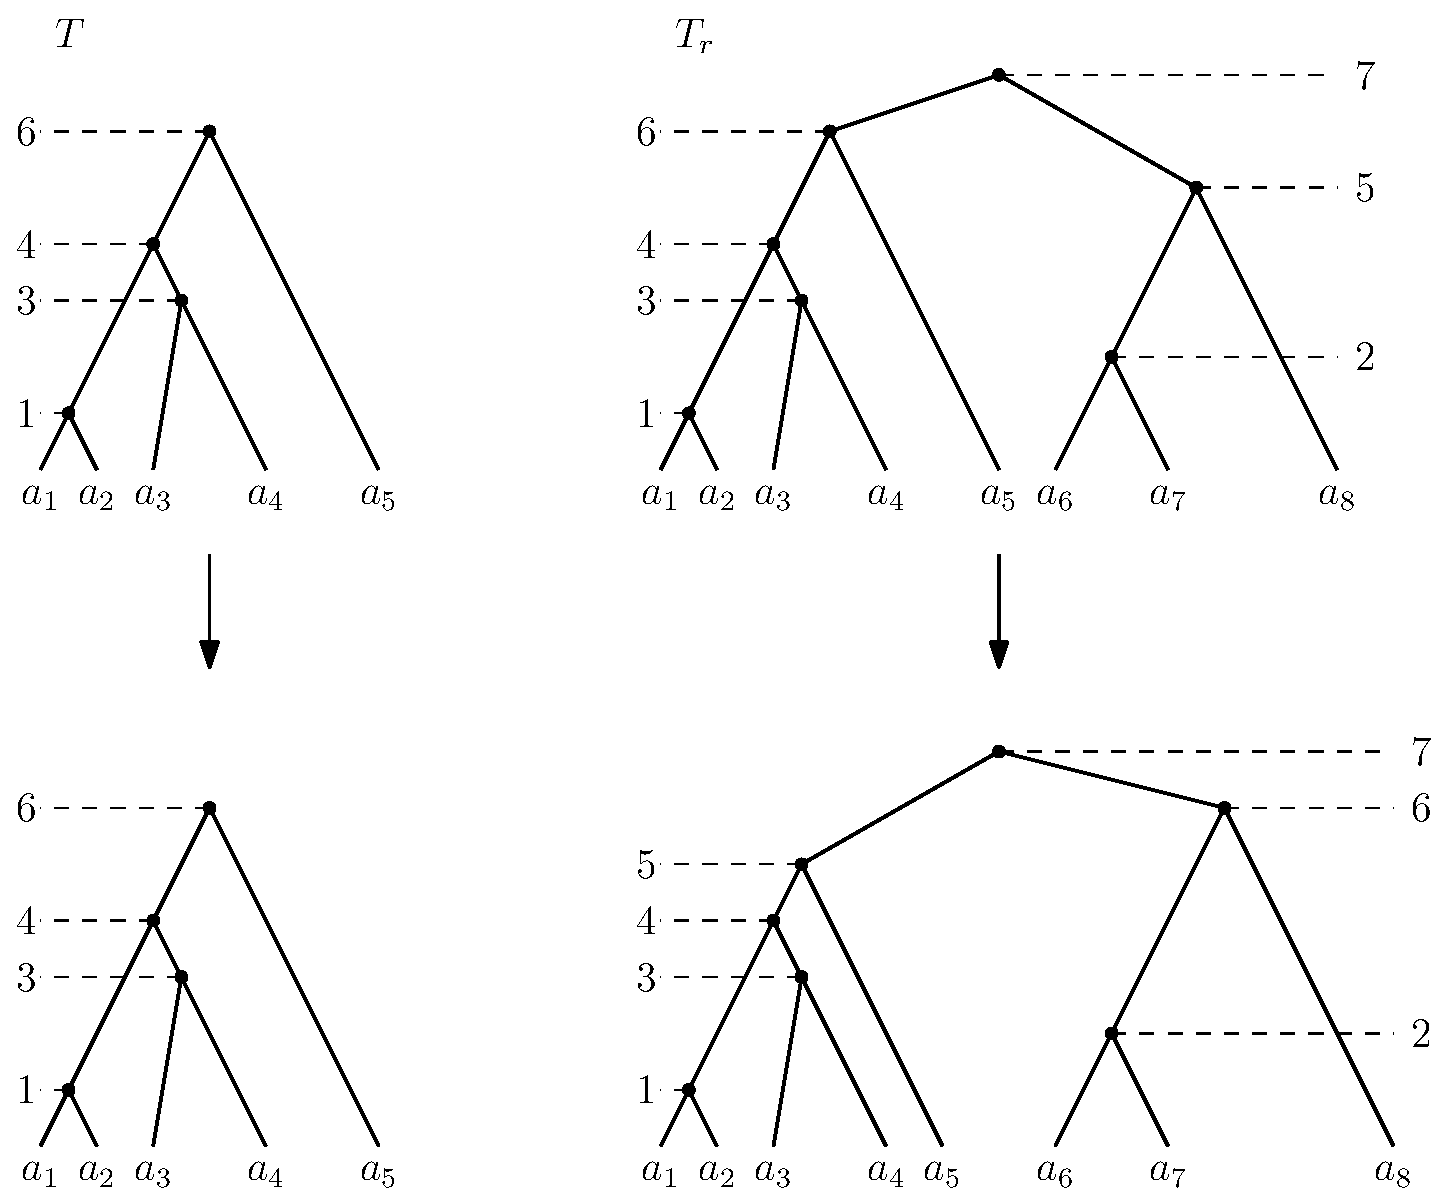
\includegraphics[width=0.75\textwidth]{dtt_to_ranked_tree.eps}
	\caption{Extending a tree $T$ on $n$ leaves in $\dtt_6$ (top left) to a ranked tree with $m+2=8$ leaves (top right) by adding a caterpillar subtree with three leaves.
	The trees on the bottom result from $T$ and $T_r$ by performing a length move (left) or rank move (right), respectively.}
	\label{fig:dtt_to_ranked_tree}
\end{figure}

\summary{Moves on the extended ranked versions of trees -- $\rnni$ vs length moves}
In the following we distinguish not only rank moves and $\nni$ moves on the extended ranked version $T_r$ of a tree $T$, but also two different types of rank moves.
Rank moves between one node of $T_r^c$ and one node of $T_r^d$ can be interpreted as length moves when considering $T_r^d$ in $\dtt_m$ (\autoref{fig:dtt_to_ranked_tree}).
Therefore, we will refer to such rank moves as \emph{rank moves corresponding to length moves}.
All remaining rank moves will still be called rank moves.
Note that the correspondence of rank moves between $T_r^c$ and $T_r^d$ to length moves in $T$ shows that any path between $T$ and $R$ in $\dtt_m$ can be interpreted as a path between $T_r$ and $R_r$ in $\rnni$.

\summary{How to compute shortest $\dtt_m$-paths between trees with $\findpath$}
After extending both trees $T$ and $R$ in $\dtt_m$ to ranked trees $T_r$ and $R_r$ on $m+2$ leaves, respectively, we can compute shortest paths between $T_r$ and $R_r$ in $\rnni$, using $\findpath$.
A path computed by $\findpath$ preserves clusters \autocite{Collienne2020-iu}, hence there are no $\nni$ moves in the newly added caterpillar subtree on the leaf set $\{a_{n+1}, \ldots, a_{m+2}\}$ on such a path.
The only moves involving internal nodes of this caterpillar subtree are rank moves that correspond to length moves, as described above.
Hence the path $\fp(T_r,R_r)$ provides a path between $T$ and $R$ in $\dtt_m$, when only considering the subtrees induced by $\{a_1, \ldots, a_n\}$ in all trees on $\fp(T_r, R_r)$, interpreting some rank moves between $T_r$ and $R_r$ as length moves.
We denote this path in $\dtt_m$, which results from $\fp(T_r, R_r)$, by $\fp(T,R)$.
In \autoref{thm:dtt_findpath} we establish that $\fp(T,R)$ is a shortest path in $\dtt_m$ indeed.
Note that for any given pair of trees $T$ and $R$, if not specified otherwise, we always assume $m$ to be the maximum root time of these trees and consider a shortest path between them in $\dtt_m$.

\begin{theorem}
	The path $\fp(T,R)$ between two discrete coalescent trees $T$ and $R$ is a shortest path in $\dtt_m$, where $m$ is the maximum root time of $T$ and $R$.
	\label{thm:dtt_findpath}
\end{theorem}

\begin{proof}
	Let $T$ and $R$ be discrete coalescent trees and $T_r$ and $R_r$ their extended ranked versions computed with \autoref{alg:ranked_tree}, respectively.
	Any path in $\dtt_m$ from $T$ to $R$ gives a path of equal length between $T_r$ and $R_r$ in the $\rnni$ space on $m+2$ leaves.
	This is due to the fact that the only moves needed in the subtree $T_r^c$ to transform it to $R_r^c$ are rank moves that correspond to length moves, and no other $\rnni$ moves.
	If there was a path between $T$ and $R$ shorter than $\fp(T,R)$, the corresponding path between $T_r$ and $R_r$ in $\rnni$ would be shorter than the one computed by $\findpath$ in this space.
	Since this contradicts the fact that $\findpath$ computes shortest paths in $\rnni$ \autocite[Theorem 1]{Collienne2020-iu}, it follows that $\fp(T,R)$ is a shortest path in $\dtt_m$.
\end{proof}

\summary{Running time of $\findpath$ + we don't need to add subtree in practice}
\autoref{thm:dtt_findpath} shows that $\findpath$ computes shortest path between two trees in $\dtt_m$ in polynomial time, more specifically in $\O(mn)$.
More details on the running time are discussed in \autoref{section:diameter} following \autoref{thm:dtt_diameter}.
It is not even necessary to convert a given pair of discrete coalescent trees to ranked trees to apply $\findpath$ to them.
Instead, we modify $\findpath$ for trees in $\dtt_m$ (\autoref{alg:fp_dtt}).
Iterations of $\findpath$ that consider clusters in the added caterpillar trees are replaced by length moves increasing the time of internal nodes as described in the \textbf{for} loop in Line~\ref{line:length_move} of \autoref{alg:fp_dtt}.
The benefit of this modified version of the algorithm, compared to using $\findpath$ on the extended ranked versions of the trees, is a reduced use of memory, which is especially of practical relevance for $m >> n$.

\begin{algorithm}[h]
	\caption{$\findpath$($T,R$)}
	\begin{algorithmic}[1]
		\label{alg:fp_dtt}
		\STATE $T_1 := T$, $p := [T_1]$
		\FOR {$k = 1, \dots, m$}
			\IF {$R$ has a node with rank $k$}
			\STATE $C:=(R)_k$
			\WHILE {$\ntime((C)_{T_1})>k$}
					\STATE $T_2$ is $T_1$ with the rank of $(C)_{T_1}$ decreased by an $\rnni$ move
				\STATE $T_1 = T_2$
				\STATE $p = p+T_1$
			\ENDWHILE
			\ELSIF {$T$ has a node with rank $k$}
				\STATE $i := \min\{l | l>k \text{ and no node in } T_1 \text{ has time }l\}$
				\FOR {$j = i-1, \dots, k$}
					\label{line:length_move}
					\STATE $T_2$ is $T_1$ where the time of $(T_1)_j$ is increased by one (length move)
					\STATE $T_1 = T_2$
					\STATE $p = p+T_1$
				\ENDFOR
			\ENDIF
		\ENDFOR
		\RETURN $p$
	\end{algorithmic}
\end{algorithm}


\section{Geometrical Properties of $\dtt_m$}
\label{section:geometry}

\subsection{Cluster Property}
\label{section:cluster_property}
\summary{Definition of Cluster Property and why it is relevant (a bit of bio).}
In this section we consider a property of tree spaces.
A tree space has the \emph{cluster property}, if all trees on every shortest paths between two trees sharing a cluster $C$ also contain this cluster.
This is a desirable biological property as trees sharing a cluster or subtree are expected to be closer to each other than to a tree not sharing a cluster with them.
An example for the practical relevance of this property are summary trees.
For a given sample of trees containing a common subtree, it is expected that their summary tree also contains this subtree.
It hence is desirable to have a tree space that has the cluster property.

\summary{Cluster property in $\nni$ and its connection to the complexity result.}
A further reason for investigating the cluster property in $\rnni$ is its importance in a similar tree space, the nearest neighbour interchange graph ($\nni$).
In the $\nni$ graph trees have no times and $\nni$ moves are allowed on every edge.
Computing distances in $\nni$ is $\np$-hard \autocite{Dasgupta2000-xa}, and the proof relies on the fact that this tree space does not have the cluster property \autocite{Li1996-zw}.
In the $\rnni$ graph, however, distances can be computed in polynomial time by $\findpath$ \autocite{Collienne2020-iu}, which preserves common clusters.
The question whether $\rnni$ has the cluster property is hence natural, and will be settled in \autoref{thm:cluster_property_rnni}.
Note that even though it seems like distances can be computed in polynomial time in a tree space if it has the cluster property, this does not need to be true in general.

\summary{$\rnni$ has the cluster property.}
\begin{theorem}
	The $\rnni$ graph has the cluster property.
	\label{thm:cluster_property_rnni}
\end{theorem}

\begin{proof}
	We assume to the contrary that there are two ranked trees $T$ and $R$ sharing a cluster $C$ and a path $p$ between these trees where $C$ is not present in every tree.
	We furthermore assume that there is no pair of trees with a shortest path not containing a shared cluster and distance less than $d(T,R)$, meaning that $T$ and $R$ give a minimum counterexample.
	Because of this minimality assumption on the length of $p$, the first tree $T'$ following $T$ on $p$ does not contain $C$.
	Since only $C$ changes by the $\nni$ move between $T$ and $T'$, all nodes with rank below $(C)_T$ induce the same clusters in $T$ and $T'$ (\autoref{fig:nni_neighbours_clusters}).
	We now compare distances $d(T,R)$ and $d(T',R)$ by using properties of $\findpath$.

	\begin{figure}[ht]
		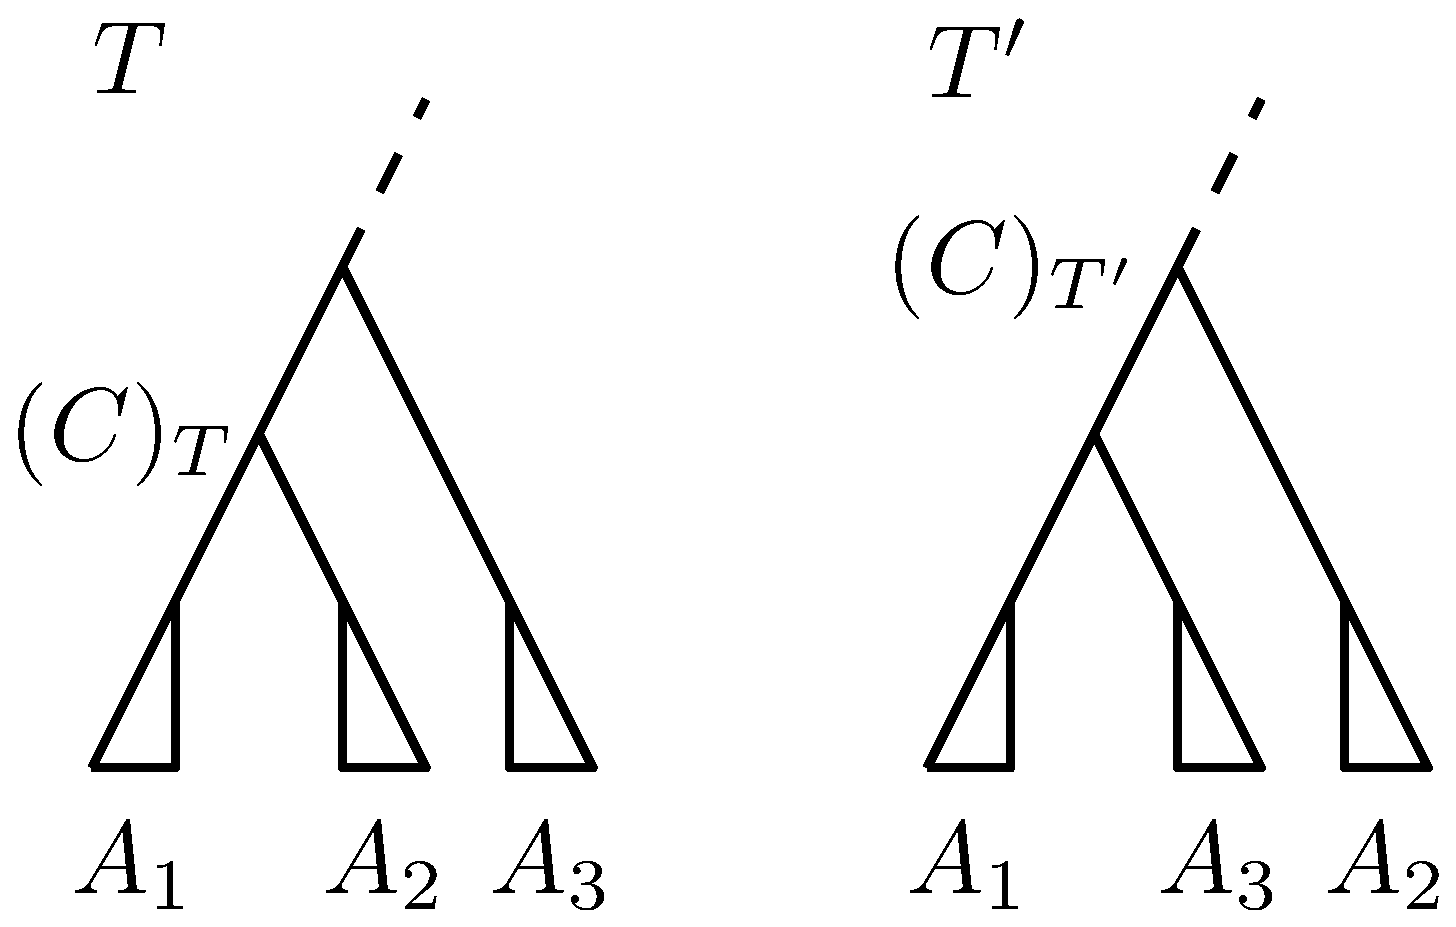
\includegraphics[width=0.33\textwidth]{nni_neighbours_clusters.eps}
		\caption{Trees $T$ and $\nni$ neighbour $T'$, such that the cluster $C = A_1 \cup A_2$ is not present in $T'$, but in $T$.}
		\label{fig:nni_neighbours_clusters}
	\end{figure}

	First we compare $\fp(R,T)$ and $\fp(R,T')$.
	All trees on on these two paths coincide until the point is reached where the cluster considered on $\fp(R,T)$ is $C$.
	Let $R'$ denote the tree at this point of the path, meaning that $\fp(R,T)$ and $\fp(R,T')$ coincide up to this tree $R'$.
	It follows $d(T,R) = d(R,R') + d(R', T)$ and $d(T',R) = d(R,R') + d(R', T')$.

	Now consider $\fp(T', R')$ to evaluate $d(R', T')$.
	As $\findpath$ preserves clusters, $C$ is present in every tree on $\fp(T,R)$ up to and including $R'$.
	The first iteration of $\findpath$ applied to the pair of trees $(T',R')$ hence considers the cluster $C$, as all cluster induced by nodes below $(C)_{T'}$ coincide in $R'$ and $T'$.
	To construct the cluster $C$ in $T'$, there is just one $\nni$ move needed, which results in the tree $T$, as $T$ and $T'$ are $\nni$ neighbours such that $T$ contains $C$ and $T'$ does not (\autoref{fig:nni_neighbours_clusters}).
	We can therefore conclude that $d(T,R) = d(T',R) - 1$, which contradicts the assumption that $T'$ is the first tree on a shortest path from $T$ to $R$.
	There is hence no shortest path between $T$ and $R$ that does not preserve $C$, which proves the cluster property for $\rnni$.
\end{proof}

The fact that a slightly modified version of $\findpath$ computes shortest paths $\dtt_m$ already suggest that shortest path in $\rnni$ and $\dtt_m$ have similar properties.
The cluster property in $\dtt_m$ follows from \autoref{thm:cluster_property_rnni}, indeed.

\begin{corollary}
	The graph $\dtt_m$ has the cluster property.
\end{corollary}

\begin{proof}
	If there was a shortest path between two trees $T$ and $R$ in $\dtt_m$ that did not preserve a common cluster, this path can be seen as a path between $T_r$ and $R_r$, the extended ranked versions of $T$ and $R$ in $\rnni$, as already discussed in \autoref{thm:dtt_findpath}.
	Since this path has the same length as the one between $T_r$ and $R_r$, it is a shortest path in $\rnni$ as well, which leads to a contradiction to \autoref{thm:cluster_property_rnni}.
\end{proof}

\subsection{Caterpillar Trees}
\label{section:caterpillar_convex}

\summary{Defining Caterpillar trees. Why are they interesting?}
In this subsection we focus on the set of caterpillar trees and establish some properties of shortest paths between those trees in both $\rnni$ and $\dtt_m$.
A path between two caterpillar trees only consisting of caterpillar trees is a \emph{caterpillar path}.
In \autoref{thm:caterpillar_convex_dtt} and \autoref{cor:caterpillar_convex_rnni} we will see that, in both $\dtt_m$ and $\rnni$, any two caterpillar trees are connected by a shortest path that is a caterpillar path.
We say that a set of trees is \emph{convex} in a tree space, if shortest paths between trees in this set stay within the set.
This is another property of $\rnni$ that the $\nni$ space of unranked trees does not have \autocite{Gavryushkin2018-ol}.
Based on the convexity of the set of caterpillar trees in $\rnni$ we introduce a way to compute distances between caterpillar trees in this space in time $\O(n \sqrt{\log n})$ in \autoref{cor:caterpillar_distance_rnni_nlogn}, and hence with better worst-case time complexity than $\findpath$.

\begin{theorem}
	The set of caterpillar trees is convex in $\dtt_m$.
	\label{thm:caterpillar_convex_dtt}
\end{theorem}

\begin{proof}
	Let $T$ and $R$ be two caterpillar trees in $\dtt_m$.
	We prove the theorem by showing that there is a caterpillar tree $T'$ that is neighbour of $T$ and closer to $R$ than $T$.
	The existence of a shortest path consisting only of caterpillar trees between $T$ and $R$ follows inductively.
	Throughout this proof we consider the extended ranked versions $T_r$ and $R_r$ of $T$ and $R$.

	Let $a_k := \argmax_{a_1, \ldots, a_n}\{\rank(a_i)_{R_r} | \rank(a_i)_{R_r} \neq \rank(a_i)_{T_r}\}$ be the leaf with parent with maximum rank in $R_r$ among those that are not in the same position in $T_r$ and $R_r$.
	Let furthermore $a_j \in \{a_1, \ldots, a_{m+2}\}$ be a leaf with $\rank(a_j)_{T_r} = \rank(a_k)_{T_r} + 1$.
	We define $T'_r$ to be the caterpillar tree resulting from $T_r$ by an $\nni$ move or rank move exchanging the ranks of $(a_k)_{T_r}$ and $(a_j)_{T_r}$.
	An $\nni$ move is necessary if these two nodes are connected by an edge, otherwise a rank move corresponding to a length move is performed on $T_r$ to receive $T'_r$ (\autoref{fig:caterpillar_convex}).
	In both cases $T'_r$ is a caterpillar tree.
	By using properties of shortest paths computed by $\findpath$, we now show that $|\fp(R_r,T'_r)| = |\fp(R_r,T_r)| - 1$.

	\begin{figure}[ht]
		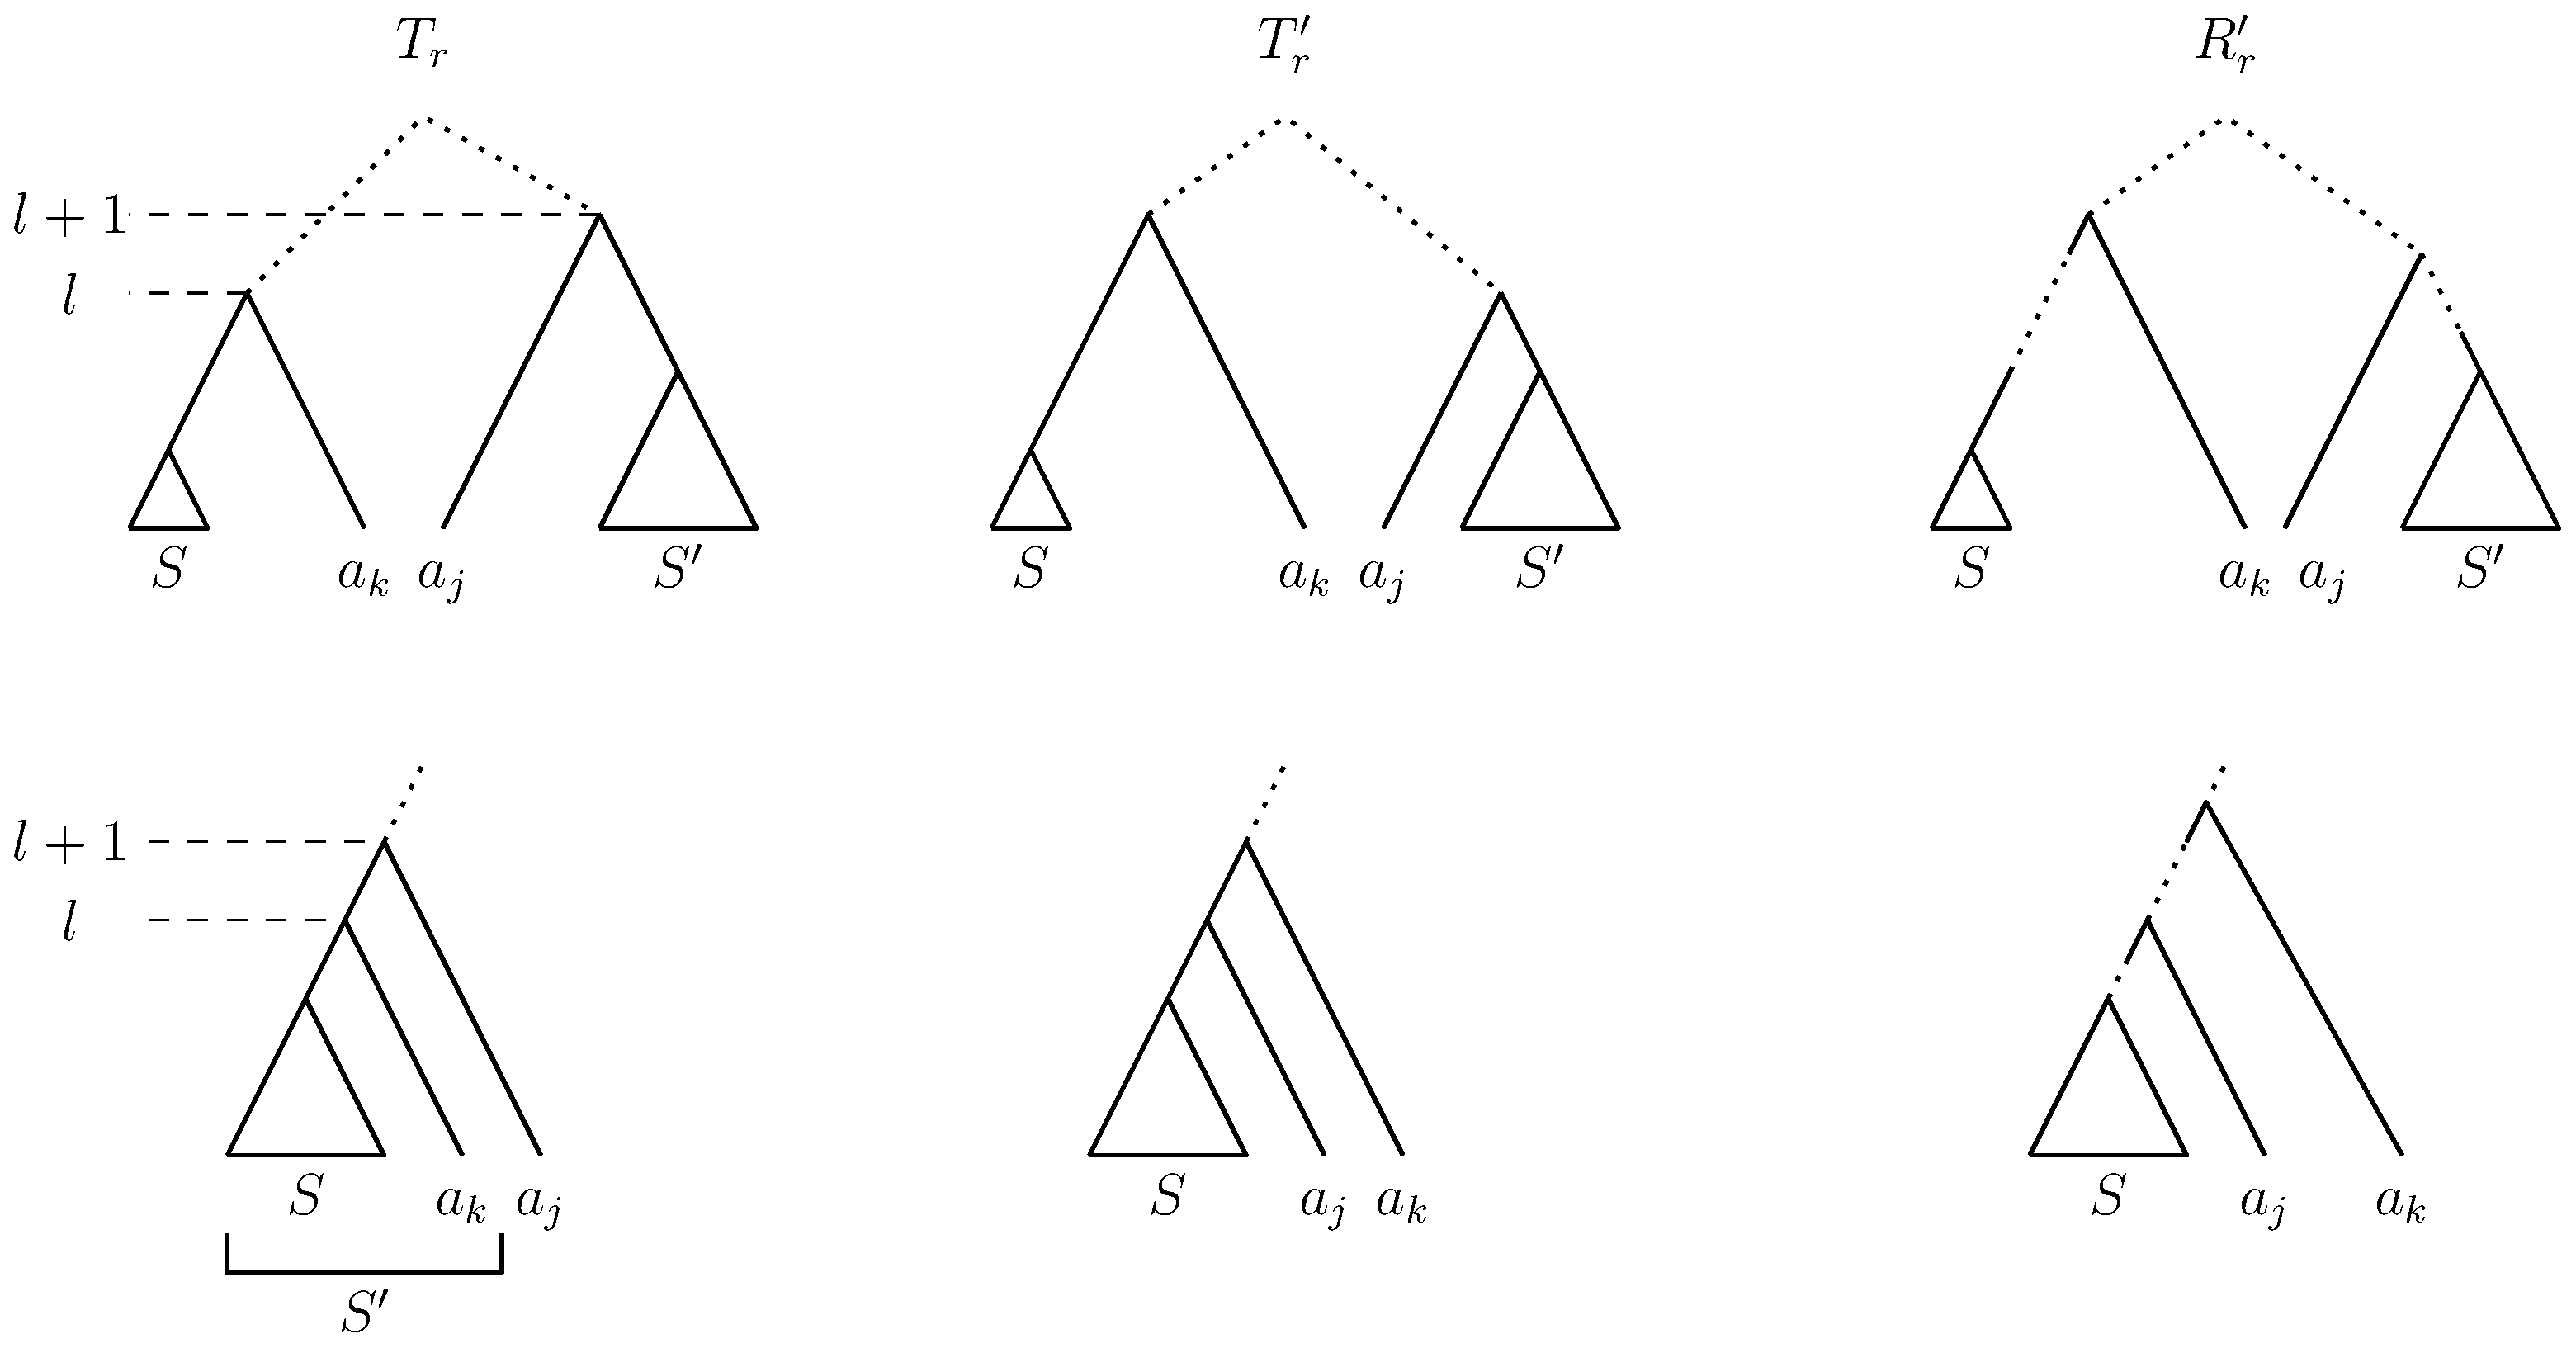
\includegraphics[width=0.66\textwidth]{caterpillar_convex.eps}
		\caption{The two possible versions of trees $T_r$ (left) and $T'_r$ (right) as described in the proof of \autoref{thm:caterpillar_convex_dtt}.
		Between $T_r$ and $T'_r$ only the parents of $a_j$ and $a_k$ are exchanged.
		At the bottom $(a_j)_T$ is parent of $(a_k)_T$, at the top these nodes are in the two different subtrees $T_r^d$ and $T_r^c$.
		Dashed lines represent remaining part of trees, which are equal in $T_r$ and $T'_r$.}
		\label{fig:caterpillar_convex}
	\end{figure}

	Since all clusters of $T_r$ and $T'_r$ induced by nodes of rank less than $\rank(a_k)_{T_r}$ coincide, the paths $\fp(R_r,T_r)$ and $\fp(R_r,T'_r)$ coincide up to a ranked tree $R'_r$, which contains all these clusters.
	We now compare the lengths of $\fp(R'_r,T_r)$ and $\fp(R'_r,T'_r)$.
	Therefore, we note at first that it is $\rank(a_j)_{R_r} < \rank(a_k)_{R_r}$ by the choice of $a_k$, and therefore also $\rank(a_j)_{R'_r} < \rank(a_k)_{R'_r}$.

	By our assumptions on $T_r$, the clusters considered on $\fp(R_r,T_r)$ in the two iterations following $R'_r$ are first $S \cup \{a_k\}$ and then $S' \cup \{a_j\}$ for some clusters $S$ and $S'$ that are present in $T_r$, $T'_r$, and $R'_r$.
	Let $l = \rank(S \cup \{a_k\})_{T_r}$ be the number of the iteration of $\fp(R_r, T_r)$ following $R'_r$.
	Decreasing the rank of $(S \cup \{a_k\})_{R'_r}$ takes $\rank(S \cup \{a_k\})_{R'_r} - l$ $\rnni$ moves.
	Because the rank of $(S \cup \{a_j\})_{R'_r}$ increases by one when the parents of $a_k$ and $a_j$ swap ranks in this iteration, the following iteration for $S' \cup \{a_j\}$ needs $\rank(S' \cup \{a_j\})_{R'_r} + 1 - (l+2)$ $\rnni$ moves.
	On $\fp(R_r,T'_r)$ however, first $\rank(S' \cup \{a_j\})_{R'_r} - l$ $\rnni$ moves decrease the rank of $(S' \cup \{a_j\})_{R'}$, and then $\rank(S \cup \{a_k\})_{R'_r} - (l+1)$ are needed for $S \cup \{a_k\}$.
	In total, for both iterations one more move is needed on $\fp(R_r, T'_r)$ compared to $\fp(R_r, T_r)$.

	The only difference in the trees after these two iterations on the two different paths is the order of ranks of the parents of $a_j$ and $a_k$.
	Since the rest of $T_r$ and $T'_r$ coincide, the remaining parts of $\fp(R_r, T_r)$ and $\fp(R_r, T'_r)$ consist of the same moves.
	With our previous observation we can conclude $d(R_r,T_r) = d(R_r,T'_r) + 1$, and hence $T'_r$ is on a shortest path from $T_r$ to $R_r$.
\end{proof}

The convexity of the set of caterpillar trees in $\rnni$ follows from the convexity of this set in $\dtt_m$ for $m = n-1$ (\autoref{thm:caterpillar_convex_dtt}).

\begin{corollary}
	The set of caterpillar trees is convex in $\dtt_m$.
	\label{cor:caterpillar_convex_rnni}
\end{corollary}

\summary{With \autoref{cor:caterpillar_convex_rnni} we can find a more efficient way to compute distances between caterpillar trees.}
Using the convexity of the set of caterpillar trees (\autoref{cor:caterpillar_convex_rnni}) in $\rnni$, there are several algorithms for computing the distance between two caterpillar trees, as the problem of computing a shortest caterpillar path can be interpreted in a few different ways.

One problem analogous to the shortest path problem for caterpillar trees is the \emph{Token Swapping Problem} (TSP) \autocite{Kawahara2017-ey} on a special class of graphs, so-called lollipop graphs.
The only moves possible between caterpillar trees in $\rnni$ are $\nni$ moves, which simply swap two leaves.
These moves can be translated to swapping two tokens in TSP.
\textcite{Kawahara2017-ey} provide an algorithm for TSP on lollipop graphs, which can be used for computing distances between caterpillar trees in $\rnni$ as well.
This algorithm however has worst-case time complexity $\O(n^2)$, the same as $\findpath$.

In the following we present an algorithm for computing distances between caterpillar trees with better worst-case time complexity, $\O(n \sqrt{\log n})$, for $\rnni$ (\autoref{cor:caterpillar_distance_rnni_nlogn}).
Therefore, we first establish a formula to express distances between two caterpillar trees in $\rnni$ (\autoref{thm:caterpillar_distance_formula}).

\begin{theorem}
	Let $T$ and $R$ be caterpillar trees in $\rnni$ such that \[1 = \rank(a_1)_R = \rank(a_2)_R < \rank(a_3)_R < \ldots < \rank(a_n)_R = n-1\]
	and
	\[P_T := \{(a_i,a_j)| \rank(a_i)_T < \rank(a_j)_T \text{ and } \rank(a_i)_R > \rank(a_j)_R\},\]
	\begin{align*}
		M_T := &\{a_i| (\forall l \textnormal{ with } \rank(a_l)_T \leq \rank(a_i)_T: \rank(a_l)_R > \rank(a_i)_r)\} \\
		& \cap \{a_i | \rank(a_i)_T < \min\{\rank(a_1)_T, \rank(a_2)_T\}\}
	\end{align*}
	Then it is
	\[d(T,R) = p_T - m_T,\]
	for ${m_T = |M_T|}$ and ${p_T = |P_T|}$.
	\label{thm:caterpillar_distance_formula}
\end{theorem}

We refer to pairs $(a_i,a_j) \in P_T$, as defined in \autoref{thm:caterpillar_distance_formula}, as transpositions.
The reason for this is that caterpillar trees can be seen as permutations of the set $\{a_1, \ldots, a_n\}$, ordered according to increasing rank of their parents.
The tree $R$ of the theorem then corresponds to the identity permutation $(a_1, a_2, a_3, \ldots, a_n)$.
Note that there is no one-to-one correspondence between permutations and caterpillar trees.
For example the permutation $(a_2, a_1, a_3, \ldots, a_n)$ corresponds to the tree $R$ as well, as the first two elements share a parent in the caterpillar tree and are hence incomparable.
Therefore, the two pairs of leaves that sharing their parent in $T$ and $R$, respectively, are not in the set $P_T$.

\begin{proof}
	Let $T$ and $R$ be caterpillar trees as described above and $\hat d(T,R) = p_T - m_T$.
	For proving $\hat d(T,R) = d(T,R)$, it is sufficient to show that for all caterpillar trees $T'$ that are neighbour of $T$ it is
	\begin{align}
		\hat d(T',R) \geq \hat d(T,R) - 1.
		\label{eq:distance_proof}
	\end{align}
	That $\hat d$ and $d$ coincide follows by induction, as in \autocite[Theorem 1]{Collienne2020-iu}.

	For proving Inequality~\ref{eq:distance_proof} we first establish $p_{T'} \geq p_T - 1$ and then $m_{T'} \leq m_t + 1$, assuming that $T'$ is a caterpillar tree that is $\rnni$ neighbour of $T$.
	We then show that it cannot be $p_{T'} = p_T - 1$ and $m_{T'} = m_T + 1$ at the same time, which proves Inequality~\ref{eq:distance_proof}.

	At most one transposition of $T$ can be resolved in $T'$, because the only move possible between caterpillar trees $T$ and $T'$ is an $\nni$ move exchanging two leaves.
	It hence is $p_{T'} \geq p_T - 1$.
	Let $a_k$ and $a_j$ be the leaves that exchange their position between $T$ and $T'$, such that $\rank(a_k)_T < \rank(a_j)_T$.
	Since these are the only leaves that change positions between $T$ and $T'$, they are the only elements that could be in $M_{T'} \setminus M_T$.
	It remains to show $(M_{T'} \setminus M_T) \neq \{a_k, a_j\}$, from which we can follow that $m_{T'} \leq m_T - 1$.
	We prove this by showing that if $a_k \in (M_{T'} \setminus M_T)$, it follows $a_j \notin M_{T'}$.

	We assume that $a_k \in (M_{T'} \setminus M_T)$, implying $a_k \notin M_T$, so at least one of the following conditions must be violated for $i = k$:
	\setcounter{equation}{0} % Set counter for equation to get C1 and C2 for conditions
	\renewcommand{\theequation}{C\arabic{equation}}
	\begin{align}
		\forall l \text{ with } \rank(a_l)_T \leq \rank(a_i)_T: \rank(a_l)_R > \rank(a_i)_R \label{condition1}\\
		\rank(a_i)_T < \min\{\rank(a_1)_T, \rank(a_2)_T\}.
		\label{condition2}
	\end{align}
	% reset counter for future uses
	\setcounter{equation}{1}
	\renewcommand{\theequation}{\arabic{equation}}

	At first we consider the case that (\ref{condition1}) is violated for $a_k$ in $T$.
	Then there is an $l$ such that $\rank(a_l)_T \leq rank(a_k)_T$ and $\rank(a_k)_R > \rank(a_l)_R$.
	It immediately follows that the same condition is violated for $a_k$ in $T'$, because the $\nni$ move exchanging $a_k$ and $a_j$ preserves the relationship of $a_k$ and $a_l$.
	It hence is $a_k \notin M_{T'}$, contradicting our assumption $a_k \in (M_{T'} \setminus M_T)$.

	We can therefore assume that (\ref{condition2}) is violated for $a_k$ to not be in $M_T$.
	It follows $\rank(a_k)_T \geq \min\{\rank(a_1)_T, \rank(a_2)_T\}$.
	As only $a_k$ and $a_j$ exchange between $T$ and $T'$ and $a_k \in M_{T'}$, it follows $a_j \in \{a_1, a_2\}$.
	This however results in a violation of (\ref{condition2}) for $a_j$ in $T'$ and hence $a_j \notin M_{T'}$.
	We can conclude $(M_{T'} \setminus M_T) \neq \{a_k, a_j\}$, and hence $m_{T'} \leq m_T + 1$.

	It remains to show that it cannot be $p_{T'} = p_T - 1$ and $m_{T'} = m_T + 1$ at the same time, in order to prove Inequality~\ref{eq:distance_proof}.
	We assume $p_{T'} = p_T - 1$, hence $(a_k,a_j)$ is a transposition in $T$, meaning that $\rank(a_k)_T < \rank(a_j)_T$ and $\rank(a_k)_R > \rank(a_j)_R$.
	As $a_k$ and $a_j$ are the only leaves that could be in $M_{T'} \setminus M_T$, it suffices to show that none of them actually are in $M_{T'} \setminus M_T$, resulting in $m_{T'} < m_T + 1$.

	That $a_k$ is not in $M_{T'}$ follows from the violation of (\ref{condition2}) by $\rank(a_j)_{T'} < \rank(a_k)_{T'}$ and $\rank(a_j)_R < \rank(a_k)_R$.
	It hence is $a_k \notin M_{T'} \setminus M_T$.
	Moreover, if $a_j \in M_{T'}$, it follows $a_j \in M_T$ as explained in the following.
	If $a_j \in M_{T'}$, both conditions (\ref{condition1}) and (\ref{condition2}) are met by $a_j$ in $T'$.
	With $\rank(a_k)_T < \rank(a_j)_T$ and $\rank(a_k)_R > \rank(a_j)_R$ it immediately follows that these conditions are also met in $T$, and hence $a_j \in M_T$, and therefore $a_j \notin M_{T'} \setminus M_T$.

	Concluding, it is $M_{T'} \setminus M_T = \emptyset$, and we can follow that if $p_{T'} = p_T - 1$, it is $m_{T'} < m_T + 1$, which concludes this proof.
\end{proof}

\begin{corollary}
	The distance between two caterpillar trees can be computed in $\O(n \sqrt{\log n})$ in $\rnni$.
	\label{cor:caterpillar_distance_rnni_nlogn}
\end{corollary}

\begin{proof}
	By \autoref{thm:caterpillar_distance_formula} the distance between two caterpillar trees in $\rnni$ is the number of transpositions between two sequences of length $n$ minus $m_T$ as defined in \autoref{thm:caterpillar_distance_formula}.
	The value $m_T$ can be computed in time linear in $n$ for any caterpillar tree $T$ by considering the leaves of the tree ordered according to increasing rank of their parents.
	The number of transpositions of a sequence of length $n$ (Kendall-tau distance) can be computed in time $\O(n \sqrt{\log n})$ \autocite{Chan2010-ls}.
	This number is equivalent to $p_T$, as defined in \autoref{thm:caterpillar_distance_formula}, when ignoring transpositions for the pairs of leaves sharing a parent in $T$ and $R$, respectively.
	The worst-case running time for computing the $\rnni$ distance between caterpillar trees is therefore $\O(n \sqrt{\log n})$.
\end{proof}

\subsection{Diameter and Radius}

\label{section:diameter}
\summary{Definition of Diameter.}
In this section we  investigate the \emph{diameter} of $\rnni$ and $\dtt_m$, which is the greatest distance between any pair of trees in each of these graphs, respectively, i.e. $\max\limits_{\text{trees }T,R}d(T,R)$.
We first establish the exact diameter of $\rnni$, improving the upper bound $n^2 - 3n - \frac{5}{8}$ given by \textcite{Gavryushkin2018-ol}.
Afterwards, we generalise this result to $\dtt_m$.

\begin{theorem}
	The diameter of $\rnni$ is $\frac{(n-1)(n-2)}{2}$.
	\label{thm:diameter_rnni}
\end{theorem}

\begin{proof}
	For proving this theorem we use the fact that $\findpath$ computes shortest paths in $\rnni$.
	Each iteration $i$ of $\findpath$, applied to two ranked trees $T$ and $R$, decreases the rank of the most recent common ancestor of a cluster $C$, induced by the node of rank $i$ in $R$, in the currently last tree $T'$ on the already computed path (starting wth $T' = T$).
	The maximum rank of $(C)_{T'}$ at the beginning of iteration $i$ is $n-1$, the rank of the root.
	As every move decreases the rank of $(C)_{T'}$ by one, there are at most $n-1-i$ moves in iteration $i$.
	The maximum length of a shortest path in $\rnni$ is hence $\sum \limits_{i = 1}^{n-1} i = \frac{(n-1)(n-2)}{2}$.
	Note that the caterpillar trees $[\{a_1, a_2\}, \{a_1, a_2, a_3\}, \ldots, \{a_1, \ldots, a_n\}]$ and $[\{a_n, a_{n-1}\}, \{a_n, a_{n-1}, a_{n-2}\}, \ldots, \{a_n, \ldots, a_1\}]$ provide an example of trees that have distance $\frac{(n-1)(n-2)}{2}$, as already pointed out in \autocite[Corollary 1]{Collienne2020-iu}, proving that this upper bound for the length of a shortest path is tight.
\end{proof}

\begin{theorem}
	The diameter of $\dtt_m$ is $\frac{(n-1)(n-2)}{2} + (m-n+1)(n-1)$.
	\label{thm:dtt_diameter}
\end{theorem}

\begin{proof}
	In order to prove the diameter of $\dtt_m$, we consider the longest path that $\findpath$ can compute between any two trees $T$ and $R$, as in the proof of \autoref{thm:diameter_rnni}.
	More specifically, we consider the maximum number of moves that $\findpath$ can perform on the extended ranked versions $T_r$ and $R_r$ of any two trees $T$ and $R$.
	Therefore, we distinguish $\rnni$ moves in the subtrees on the leaf set $\{a_1, \ldots, a_n\}$ from the rank moves that correspond to length moves, i.e. rank moves between one node of each of the subtrees on leaf subsets $\{a_1, \ldots, a_n\}$ and $\{a_{n+1}, \ldots a_{m+2}\}$.

	The maximum number of $\rnni$ moves (excluding rank moves that correspond to length moves) on $\fp(T_r,R_r)$ follows from \autoref{thm:diameter_rnni} and is $\frac{(n-1)(n-2)}{2}$.
	To establish the maximum number of rank moves that correspond to length moves on a shortest path between $T_r$ and $R_r$ is reached when every internal node of the subtree $T_r^c$ of $T_r$ swaps rank with every internal node of the subtree $T_r^d$.
	The maximum number of such rank swaps corresponding to length moves is hence $(m-n+1)(n-1)$.

	The sum of the maximum number for $\rnni$ and length moves is therefore $\frac{(n-1)(n-2)}{2} + (m-n+1)(n-1)$.
	That this upper bound is actually the diameter of $\dtt_m$ can be proven by the trees $T$ and $R$ in \autoref{fig:cat_max_dist_dtt} for which the path computed by $\findpath$ has length $\frac{(n-1)(n-2)}{2} + (m-n+1)(n-1)$.
	Both $T$ and $R$ are caterpillar trees and defined by
	\[m-n-1 = \rank(a_1)_T = \rank(a_2)_T < \rank(a_3)_T < \ldots < \rank(a_n)_T = m\]
	and
	\[1 = \rank(a_1)_R = \rank(a_n)_R < \rank(a_{n-1})_R < \ldots < \rank(a_1)_R = n-1.\]
	\begin{figure}[ht]
		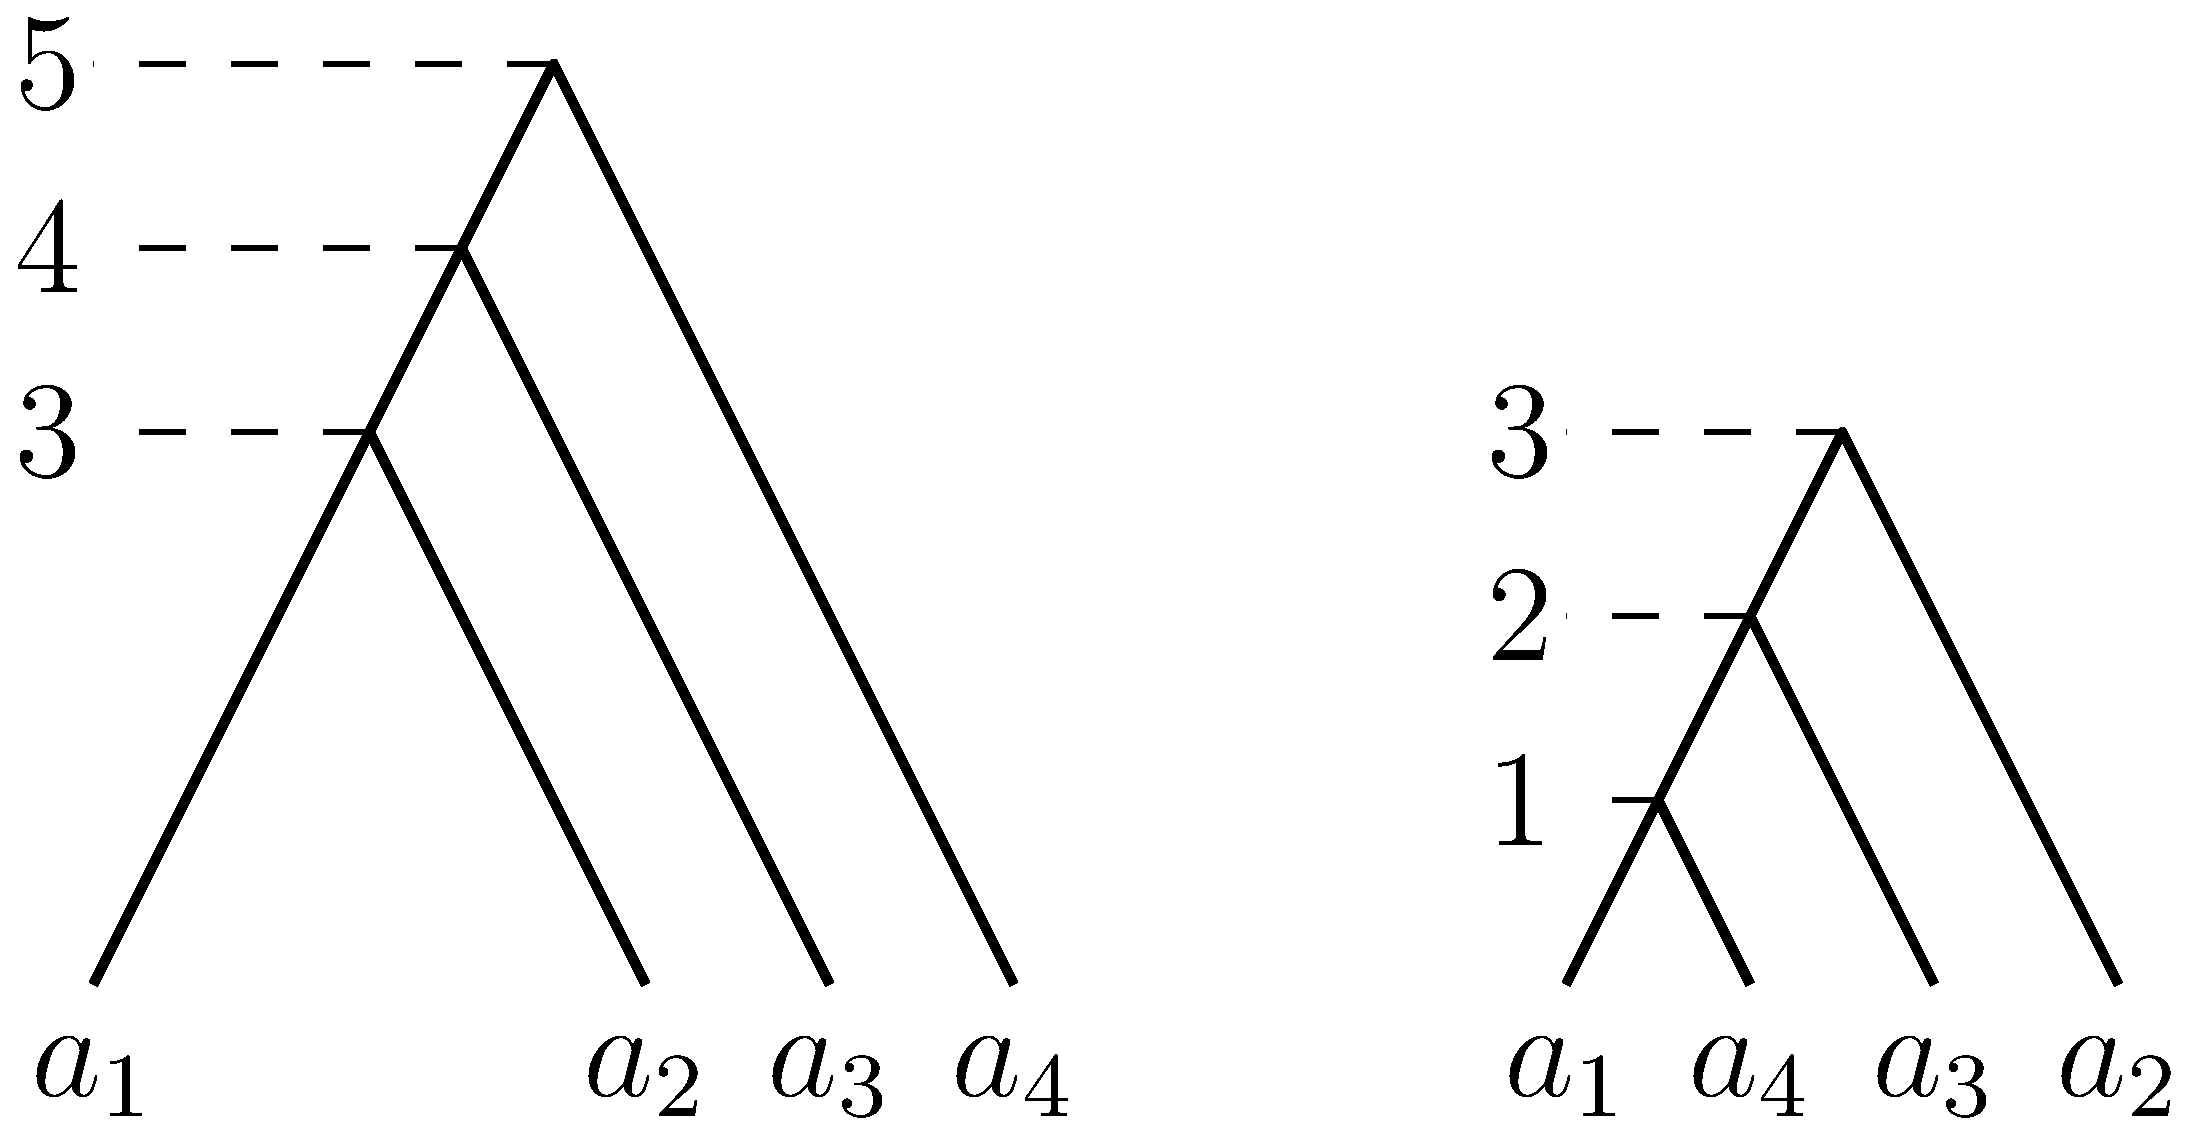
\includegraphics[width=0.65\textwidth]{cat_max_dist_dtt.eps}
		\caption{Trees $T$ and $R$ with distance $\frac{(n-1)(n-2)}{2} + (m-n+1)(n-1)$ as described in the proof of \autoref{thm:dtt_diameter}}
		\label{fig:cat_max_dist_dtt}
	\end{figure}
\end{proof}

Note that the worst-case running time of $\findpath$ is $\O(n^2)$ in $\rnni$ and $\O(nm)$ and $\dtt_m$ and depends on the diameter of the corresponding tree spaces.
For computing a shortest path, there is no algorithm with better worst-case running time than this, as the running time for algorithms computing shortest paths is bounded from below by the diameter of the corresponding space.
There can however be more efficient algorithms for just computing distances.

\summary{Radius of $\rnni$ is equal to its diameter.}
The \emph{radius} of a graph is defined as he minimum distance of any vertex in the graph to the vertex with maximum distance from it.
For $\dtt_m$ and $\rnni$, this is $\min\limits_{\text{tree } T}\max\limits_{\text{tree }R} d(T,R)$, where $d$ is the distance measure in the corresponding graph.
In the following we see that the radius of $\rnni$ equals its diameter, which is not true for $\dtt_m$, as we will see afterwards.

\begin{theorem}
	The radius of $\rnni$ equals its diameter $\frac{(n-1)(n-2)}{2}$.
	\label{thm:radius_rnni}
\end{theorem}

\begin{proof}
	We prove this lemma by showing that every ranked tree $T$ in $\rnni$ has a caterpillar tree $R$ with distance $\frac{(n-1)(n-2)}{2}$ to $T$, using induction on the number of leaves $n$.

	The base case $n=3$ is trivial, as all three trees in this space are caterpillar trees with distance one from each other.
	For the induction step we consider an arbitrary tree $T$ with $n+1$ leaves.
	Let $x$ and $y$ be the leaves of $T$ that share the internal node of rank one as parent in $T$, and let $T_{n-1}$ be the tree on $n$ leaves resulting from deleting one of these leaves, say $x$, of $T$.
	By the induction hypothesis there is a caterpillar tree $R_{n-1}$ with distance $\frac{(n-1)(n-2)}{2}$ to $T_{n-1}$.
	Now consider the tree $R$ resulting from adding $x$ at the top of $R_{n-1}$ such that the root of $R$ has $x$ and $R_{n-1}$ as children.

	We now consider $\fp(R,T)$.
	In the first iteration of $\findpath$, $(\{x,y\})_R$ moves down until it reaches rank one.
	Therefore, first $(x)_R$ moves down by $\nni$ moves until it reaches rank $\rank(y)_R + 1$.
	Then a further $\nni$ move creates an internal node with children $x$ and $y$, before this node is moved down by rank swaps to reach rank one as depicted in Figure~\ref{fig:max_dist_ctree}.
	Altogether, there are $n-1$ $\rnni$ moves needed in the first iteration, as the rank of the parent of $x$ decreases by one within every move, starting at the root with rank $n$ and ending at the internal node of rank one.
	The tree at the end of this first iteration on $\fp(R,T)$ is identical to $R_{n-1}$ when removing the leaf $x$ and suppressing its parent (the node of rank one).
	Since the cluster $\{x,y\}$ is not considered again in $\findpath$, the remaining part of $\fp(R,T)$ contains the same moves as $\fp(R_{n-1},T_{n-1})$, and hence $|\fp(R,T)| = |\fp(R_{n-1},R_{n-1})| + n-1$.
	Therefore it is $d(T,R) = \frac{(n-1)(n-2)}{2} + n-1 = \frac{n(n-1)}{2}$, which proves the lemma.
	\begin{figure}[ht]
		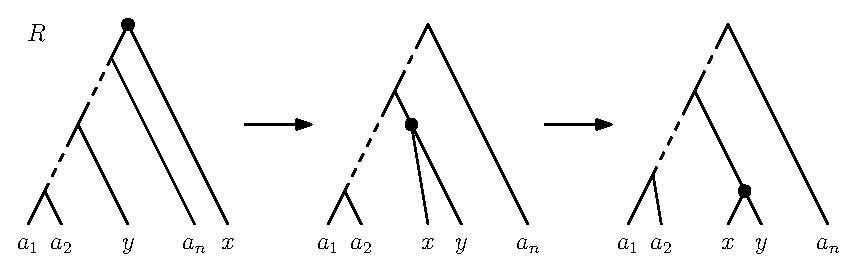
\includegraphics[width=0.8\textwidth]{max_dist_ctree.eps}
		\caption{Initial $n - 1$ $\rnni$ moves of $\fp(R,T)$ as described in the proof of Lemma~\ref{thm:radius_rnni}.
		Removing the leaf $x$ and suppressing the non-root node of degree two from the tree on the right results in $R_{n-1}$ as described in the lemma.}
		\label{fig:max_dist_ctree}
	\end{figure}
\end{proof}

Unlike in $\rnni$, the radius of $\dtt_m$ does not equal its diameter.
A counterexample is given by the tree depicted in \autoref{fig:dtt_radius_counterexample} on three leaves in $\dtt_4$.
There is no tree in $\dtt_4$ that has distance $\frac{(n-1)(n-2)}{2} + (m-n+1)(n-1)$ (diameter of $\dtt_m$) from that tree.

\begin{figure}[ht]
	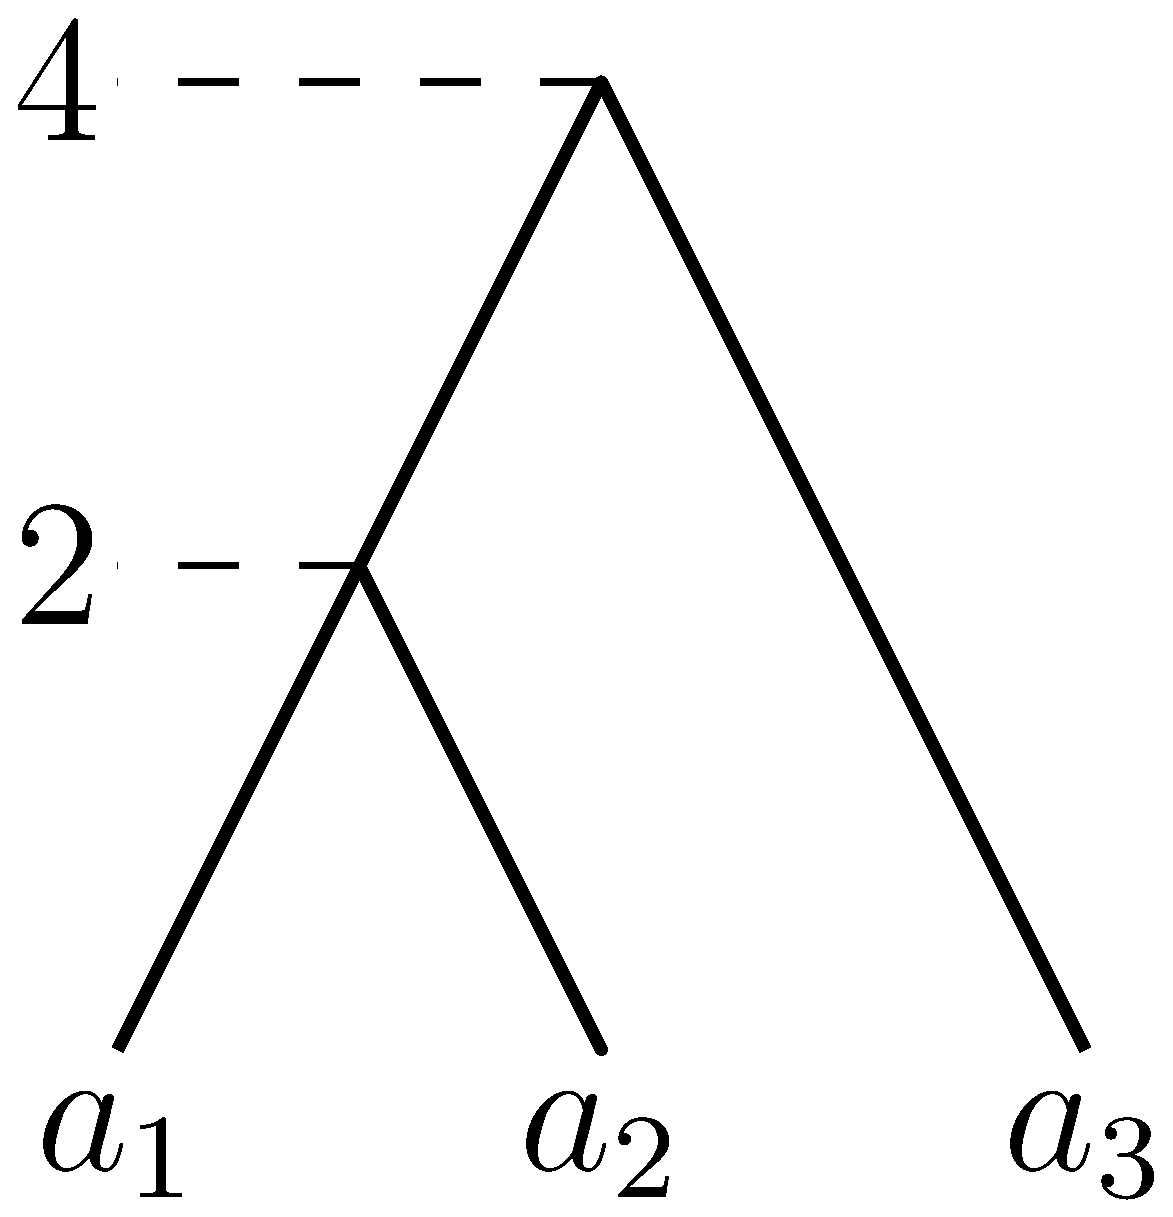
\includegraphics[width=0.15\textwidth]{dtt_radius_counterexample.eps}
	\caption{Tree in $\dtt_4$ on three leaves for which there is not tree with distance $5 = \frac{(n-1)(n-2)}{2} + (m-n+1)(n-1)$ (diameter) from it}
	\label{fig:dtt_radius_counterexample}
\end{figure}


\section{Related problems and future research questions}
\label{section:open_problems}

In this paper we introduced and analysed properties of the space of discrete coalescent trees $\dtt_m$.
An important tool for establishing these characteristics of the tree space is the algorithm $\findpath$, which has been introduced by \textcite{Collienne2020-iu} for $\rnni$.
We generalised this algorithm and showed in \autoref{thm:dtt_findpath} that it solves the shortest path problem in $\dtt_m$ as well.
Afterwards, we established properties of $\dtt_m$ and $\rnni$ such as the cluster property (\autoref{section:cluster_property}), the convexity of the set of caterpillar trees (\autoref{section:caterpillar_convex}), diameter, and radius (\autoref{section:diameter}).

With the convexity of the set of caterpillar trees in $\rnni$ we also found a more efficient way of computing distances between such trees, using the correspondence between caterpillar trees and permutations.
In the following we discuss the connection of the $\rnni$ graph, not only the caterpillar subgraph, with a well-known algebraic structure, the partition lattice.
Following that, we discuss further open problems providing new ideas for future research.

\subsection{Partition Lattice}
The connection of $\rnni$ to partition lattices provides a new direction for further research and translates results and open problems from the language of phylogenetics to the language of lattice theory.

The \emph{partition lattice} on $\{1, \ldots, n\}$ is the lattice given by the partially ordered set $(\Pi_n, \leq)$, where $\Pi_n$ is the power set of $\{1, \ldots, n\}$ and $X \leq Y$ if partition $X$ refines $Y$, that is, $X \leq Y \Leftrightarrow (\forall x \in X)(\exists y \in Y) x \subseteq y$.
For simplification we will denote the partition lattice on $n$ elements by $\Pi_n$.
$\Pi_4$ is illustrated in Figure~\ref{fig:partition_lattice4}.
We assume that a partition $X$ in the partition lattice $\Pi_n$ has rank $k$ if the number of elements in $X$ is $n-k$.
The algebraic structure of $\Pi_n$ is related to the $\rnni$ graph on trees on $n$ leaves in the following way.

\begin{theorem}
The $\rnni$ graph on $n$ leaves is isomorphic to the graph of maximal chains of the partition lattice $\Pi_n$ where two maximal chains are connected by an edge if and only if they differ by exactly one partition.
The corresponding metric spaces are isometric.
\label{thm:partition_lattice}
\end{theorem}

\begin{proof}
There is a one-to-one relation between ranked trees and maximum chains in a partition lattice.
We can define a bijective mapping from the set of ranked trees to the set of maximum chains in $\Pi_n$ as follows.
A ranked tree $T$ maps onto a maximum chain $\mathcal{C}_T$ if the set in the partition of rank $i$ in $\mathcal{C}_T$ that is the union of two sets of the partition of rank $i-1$ in $\mathcal{C}_T$ is the cluster induced by the internal node of rank $i$ in $T$.

Note that this bijection is an isomorphism between the $\rnni$ graph and the graph of chains as in the theorem.
Indeed, two chains are different by exactly one partition if and only if the corresponding trees are connected by an $\rnni$ move.
\end{proof}

\begin{figure}[H]
\centering
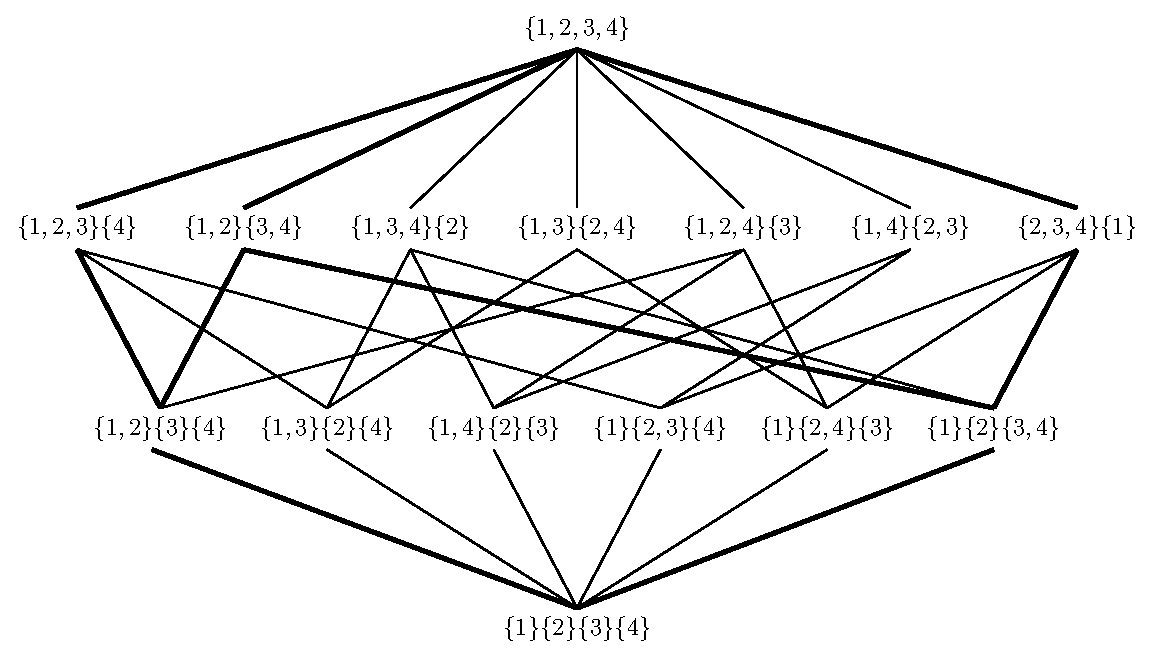
\includegraphics[width=\textwidth]{partition_lattice4}
\vspace{12pt}
\caption{The partition lattice $\Pi_4$ on $\{1,2,3,4\}$.
The highlighted edges correspond to an $\rnni$ path from the tree represented by the leftmost chain to the rightmost one.}
\label{fig:partition_lattice4}
\end{figure}

Figure~\ref{fig:partition_lattice4} is an illustration of the proof of Theorem~\ref{thm:partition_lattice}.
The four chains indicated in bold correspond to the following $\rnni$ path.
The leftmost chain corresponds to the caterpillar tree $[\{1, 2\}, \{1, 2, 3\}, \{1, 2, 3, 4\}]$ (in the cluster representation).
First, the partition $\{1, 2, 3\} \{4\}$ is replaced with $\{1, 2\} \{3, 4\}$ and we get the chain corresponding to the tree $[\{1, 2\}, \{3, 4\}, \{1, 2, 3, 4\}]$, which is one $\rnni$ move away from the caterpillar tree.
Second, the partition $\{1, 2\} \{3\} \{4\}$ is replaced with $\{1\} \{2\} \{3, 4\}$, which corresponds to the rank swap on the previous tree.
Third, the partition $\{1, 2\} \{3, 4\}$ is replaced with $\{1\} \{2, 3, 4\}$ and we reach the caterpillar tree $[\{3,4\}, \{2, 3, 4\}, \{1, 2, 3, 4\}]$.

\subsection{Further Open Problems}

\summary{Radius $\dtt_m$}
One question left open in this paper is the radius of $\dtt_m$.
We established the radius of $\rnni$ and found an example showing that this result cannot be generalised to $\dtt_m$.
Finding the radius of $\dtt_m$ is therefore one of the natural next steps for further analyses of the geometry of $\dtt_m$.

\summary{More efficient algorithm for computing distances (not shortest paths)}
The worst-case time complexity of $\findpath$ for computing a shortest path is $\O(mn)$ in $\dtt_m$.
And in \autoref{section:diameter} we have seen that there is no algorithm with better worst-case running time for computing shortest paths.
It might however be possible to compute distances more efficiently.
In fact, we established in \autoref{section:caterpillar_convex} a way for computing distances between caterpillar trees in $\O(n \sqrt{\log n})$.
This raises the question whether there is an algorithm that computes the distance between any two trees in $\dtt_m$ with better running time than $\findpath$.
\todo{Add David's result about mapping to $L_1$ here?
Yes, unless it's already somewhere.}

\summary{$\rnni(rho)$ and parameter $\rho$ for discrete coalescent trees}
Throughout this paper we consider $\dtt_m$ as a generalisation of $\rnni$ by allowing internal nodes to have integer-valued time differences.
We therefore introduced the parameter $m$ to bound the height of a tree in the space of discrete coalescent trees in order to get a finite space.
A different parameter $\rho$ has previously been introduced in \textcite{Collienne2020-iu} for generalising $\rnni$ to a space $\rnni(\rho)$ of ranked trees, where rank and $\nni$ moves have weights $\rho$ and one, respectively.
Combining these two approaches of generalising $\rnni$ gives a space of discrete coalescent trees where different moves have different weights.
This tree space is relevant for practical applications, where for example some knowledge about the tree topology exists, but the uncertainty of the timing of internal nodes remains high.
Investigating such a tree space could therefore be a next step for further studies.

\summary{scaling-free tree space}
Another due to its biological relevance important property of tree spaces is the cluster property, discussed in \autoref{section:cluster_property}.
For some applications a further property that none of the commonly used tree spaces possesses is desired.
Sometimes studies aim to compare two trees on different data sets.
The goal of such comparisons is to compare the branching process through time.
Since the given trees arise from different data sets, a scaling-free tree space is desired.
The tree space $\rnni$ and $\dtt_m$ have shortest paths computable in polynomial time, and therefore might be a good starting point for finding a scaling-free tree space where distances can be computed efficiently.

\printbibliography
\end{document}
